% !TEX root = ../master.tex
\chapter{Design and Methodology}
\label{chap:design}
This chapter describes which research method is used to design a solution 
that answers the initial questions posed in the first chapter.
The considerations that contribute to the design of this solution are outlined 
and form the foundation for its implementation in the next chapter.

\section{Employed Methodology}

Preceding to the practical part of this thesis, 
the method to follow along shall be laid out here.
One suitable method is the general concept of \emph{design science research}, also known as \emph{constructive research}, 
since it involves the development and evaluation of artifacts to solve domain specific problems.
It therefore conveys a improved practical relevance in comparison to purely descriptive research methods,
while the outcomes still create scientific knowledge
\autocite[][p.~v]{dresh2015designresearch}.
The conducted research must design an artifact, such as a construct, model or method, that solves a relevant problem in a specific field, which is evaluated regarding its utility, quality and efficacy.
The performed research should be based on rigorous scientific methods and contribute to the current theoretical body of knowledge.
The conducted design process must take into account the practical environment it is executed in and use the available resources.
A conclusion of the project for both technology-oriented as well as management-oriented audiences should be presented in the end
\autocite[][p.~70]{dresh2015designresearch}.

\begin{figure}[hbt]
	\centering
	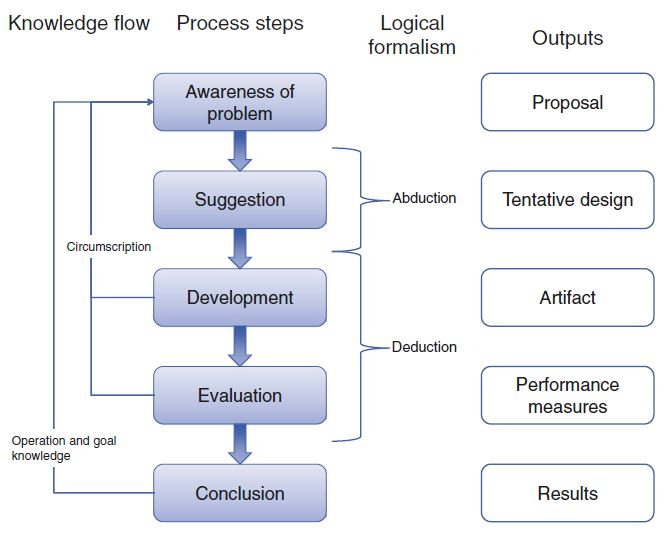
\includegraphics[width=0.8\textwidth, keepaspectratio]{resources/designscienceresearchoutputs.jpg}
	\caption{\label{fig:design:designscience} Process steps and outputs of design science research. Reprinted from \textcite[][p.~83]{dresh2015designresearch}}
\end{figure}

Figure \ref{fig:design:designscience} displays the steps that are found in the process of design science research. 
Those are the steps that guide the execution of this thesis.
The awareness and relevance for the given problem has already been given in section \vref{sec:into:context}.
Looking back to the original research questions (see section \vref{sec:intro:goals}) two focuses have been identified for this thesis:

\begin{itemize}
    \item Which computer vision techniques can be used to detect persons and objects within an elevator car and in front of the lift and estimate their spacial volume?
    \item How can the information acquired by a system that uses such methods constitute to the optimization of algorithms that control the movement plan for elevators?
\end{itemize}


To answer the two questions, the conducted research is therefore twofold.
The first part involves the design and experimental implementation of a system to gather passengers volume data in elevators.
The second part deals with the integration of this information into a scheduling algorithm.
Outlined below are the steps that are taken to
suggest a tentative design for each, develop the artifacts and evaluate them.

For the  design and implementation of a vision system to gather volume data of passengers,
the following steps are performed:

\begin{enumerate}
    \item Find a typical or actual elevator control system architecture and define the positions to integrate the necessary components for an vision system into it.
    \item Define the exact type and structure of the information that the vision system should be able to detect.
    \item Find an algorithmic approach to  passenger detection and volume estimation that is suitable to generate the required data.
    \item Match the approach with an possible hardware setup to perform tests with it.
    \item Test the proposed detection system in an real world experiment that includes  exemplary footage from within an cabin and of a lobby.
    \item Evaluate the results of the test for the functionality and effectiveness of the employed system.
\end{enumerate}

For the integration of the  passenger data into existing scheduling algorithm the following steps are performed:

\begin{enumerate}
    \item Define a suitable elevator configuration that could possibly benefit from the information that the vision system can provide. 
    Find a typical or actual control algorithm that is used for such a configuration.
    \item Adapt the scheduling algorithm to use the additional information.
    \item Compare the two versions of the algorithm in order to determine their effectiveness regarding a suitable metric.
    A simulation is used to perform this comparison.
\end{enumerate}

%\begin{figure}[hbt]
%	\centering
%	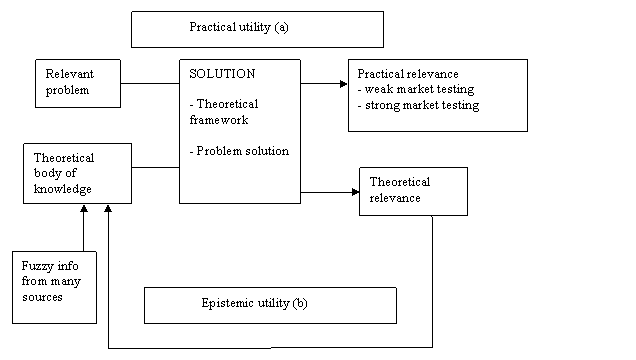
\includegraphics[width=1.0\textwidth, keepaspectratio]{resources/Rasvan_constructive_research_diagram}
%	\caption{\label{fig:design:constructiveresearch} Elements of constructive research. Source:
%	\url{https://en.wikipedia.org/wiki/File:Rasvan_constructive_research_diagram.gif}}
%\end{figure}
 
\section{Visual System}
TODO
\subsection{Proposal for Integration into Elevator Control System Architecture}
TODO
for hardware setup
- no additional sensory
- add cv system (computer) and multiple cams inside each cabin
- add cv system (computer) and multiple or one cam outside on each floor
\subsection{Output Data Definition}
TODO
- for each objects weather it is a person or an cargo object
- for each persons a volume description approximated by an innner and outer elipse (or simple: circle) and a high
- 
- total number of passengers and cargo objects inside and infront
\subsection{Detection Technique}
TODO
\subsection{Test Arrangement and Validation Strategy}
TODO

\section{Scheduling Algorithm}
TODO
\subsection{Suitable Elevator Configuration}
TODO
\subsection{Adaption of Scheduling Algorithm}
TODO
\subsection{Preparation for Simulation and Validation Strategy}
TODO
 

%\section{Requirements}
%TODO
%\autocite[][]{xang2016trafficlist} has done tehe same and patentet it :(
%\section{Conduction of Method}
%TODO the method determines which steps to take
%TODO, choose possible approach from sota
%\section{Proposed Solution}
%TODO next two are included?
%\section{Architectural Plan}
%TODO necessary? yes
%\section{Algorithmic Approach}
%TODO necessary? yes
%\section{Validation Strategy}
%TODO